\documentclass{article}
\usepackage[utf8]{inputenc}
\usepackage{amsmath}
\usepackage{amsfonts}
\usepackage{esint}
\usepackage{geometry}
\usepackage{color}
\usepackage{fancyhdr}
\usepackage{ctable}
\usepackage{fancybox}
\usepackage{tabularx}
\usepackage{array}
\usepackage{booktabs}
\usepackage[french]{babel}
\usepackage{dsfont}
\usepackage{setspace}
\usepackage[french]{minitoc}
\usepackage{multicol}
\usepackage{multirow}
\usepackage[hidelinks]{hyperref}
\usepackage{graphicx}
\usepackage[T1]{fontenc}
\usepackage{xcolor}
\usepackage{listings}

\geometry{top=2.5cm, bottom=2.5cm, left=3cm, right=3cm}

\addtocounter{tocdepth}{3}
\setcounter{secnumdepth}{3}


\definecolor{codegreen}{rgb}{0,0.6,0}
\definecolor{codegray}{rgb}{0.5,0.5,0.5}
\definecolor{codepurple}{rgb}{0.58,0,0.82}
\definecolor{backcolour}{rgb}{0.95,0.95,0.92}

\lstdefinestyle{mystyle}{
  backgroundcolor=\color{white}, commentstyle=\color{codegreen},
  keywordstyle=\color{magenta},
  numberstyle=\tiny\color{codegray},
  stringstyle=\color{codepurple},
  basicstyle=\ttfamily\footnotesize,
  breakatwhitespace=false,         
  breaklines=true,                 
  captionpos=b,                    
  keepspaces=true,                 
  numbers=left,                    
  numbersep=5pt,                  
  showspaces=false,                
  showstringspaces=false,
  showtabs=false,                  
  tabsize=2
}

\lstset{style=mystyle}

\begin{document}

%%%%%%%%%%%%%%%%%%%%%%%%%%%%%%%%%%%%%%%%%%%%%%%%%%%%%%
%%%%%%%%%%%%%%%%%%%% PRÉSENTATION %%%%%%%%%%%%%%%%%%%%
%%%%%%%%%%%%%%%%%%%%%%%%%%%%%%%%%%%%%%%%%%%%%%%%%%%%%%

\begin{titlepage}

    \unitlength 1cm
    \begin{center}
    
    \vspace*{1cm}

    
\includegraphics[scale=0.6]{figures/logo_ico.png}
    
    \vspace{2cm}
    
               {\Large Diplôme de Qualification en Physique Radiologique et Médicale\\}
               
    \vspace{2cm}           
    
    
    \rule{16cm}{0.7pt}
    
    \vspace{12pt}
               
               {\LARGE \bf Faisceaux de photons de haute énergie : cas des petits faisceaux\\}
               
    \vspace{12pt}
    \rule{16cm}{0.7pt}

    \vspace{2cm}

                {\large Fiche n°3b}
    
    \vspace{1.5cm}

               {\Large\bf {Alexandre \textsc{Rintaud}}}
    
    \vspace{1.5cm}
    
    \end{center}
    
    Encadrants :
    
    \small {
    \begin{tabular}{llr}\\
    \textbf{Stéphanie \textsc{Josset}}   &  &  \\
      Physicienne médicale, \textsc{Centre René Gauducheau ICO, Saint Herblain} &    &  \\
    
    \end{tabular}
    }

    \vspace{1.5cm}


    \begin{center}
    \textsc{Semestre 3 2024}
    \end{center}
    
\end{titlepage}
\let\cleardoublepage\clearpage


%%%%%%%%%%%%%%%%%%%%%%%%%%%%%%%%%%%%%%%%%%%%%%%%%%%%%%
%%%%%%%%%%%%%%%%%%%%%%% STYLE %%%%%%%%%%%%%%%%%%%%%%%%
%%%%%%%%%%%%%%%%%%%%%%%%%%%%%%%%%%%%%%%%%%%%%%%%%%%%%%

\onehalfspacing

%Style  du corps
\pagestyle{fancy}
	\renewcommand\headrulewidth{0.5pt}
	\renewcommand\footrulewidth{0.5pt}
	\fancyfoot[L]{\textsc{A. Rintaud}}
	\fancyfoot[C]{\textsc{ICO Nantes}}
	\fancyfoot[R]{\thepage}

\tableofcontents
\clearpage
\section{Introduction}

La radiothérapie externe utilise, de manière prépondérante, les faisceux de photons de haute énergie afin de traiter des cellules cancéreuse tout en épargnant le plus possible les tissus sains. Dans cette optique, la connaissance précise des caractéristiques dosimétriques ainsi que les incertitudes associées de l'accélérateur utilisé sont nécessaires. 

Ce rapport traitera des faisceaux de photons utilisés en radiothérapie. Premièrement, le matériel et les méthodes utilsiées lors des mesures des doses absolues basées sur les protocoles internationnaux fournis par l'Agence Internationale de l'Énergie Atomique (AIEA) seront explicités, puis les résultats seront présentés. 

\section{Matériels et méthodes}

Cette partie est consacrée à la mesure de la dose absorbée dans les conditions de référence, telles que décrites dans le protocole TRS-398 de l'AIEA. De plus, nous développerons également la méthodologie du protocole TRS-277.

\subsection{Facteurs correctifs}

L'utilisation d'une chambre d'ionnisation à cavité d'air étanche engendre une fluctuation de la réponse du système de mesure en fonction de plusieurs paramètres. Il faut donc appliquer une correction de la mesure :

\begin{equation}
  M_{Q'} = M_Q \times k_{T,P} \times k_{pol} \times k_{rec} \times k_H
  \label{eq_corr_charge}
\end{equation}

Avec $M_Q$ la charge mesurée sur l'électromètre, $k_{T,P}$ le facteur correctif de la pression et de la température, $k_{pol}$ le facteur correctif de la polarisation de la chambre, $k_{rec}$ le facteur correctif de la recombinaison ionique 

\subsubsection{Pression et température}

Le facteur $k_{T,P}$ permet de corriger de la pression et de la température et se calcule de la manière suivante :

\begin{equation}
  k_{T,P} = \dfrac{P_0T}{T_0P}
  \label{eq_k_TP}
\end{equation}

Avec $P_0$ et $T_0$ la pression et la température de référence, respectivement égales à 1013,25 hPa et 273,15 K, $P$ et $T$ sont la pression et la température de la salle lors de la mesure.

\subsubsection{Polarisation}

Ce facteur correctif, noté $k_{pol}$, permet de corriger de l'effet de la polarité appliquée à la chambre lors de la mesure

\begin{equation}
  k_{pol} = \dfrac{|M_+| + |M_-|}{2M}
  \label{eq_pol}
\end{equation}

Avec $M_+$ et $M_-$ les charges mesurées pour les tensions $V_+$ et $V_-$ respectivement et $M$ est la réponse pour la tension utilisée en clinique.

\subsubsection{Recombinaisons ioniques}

Le facteur de recombinaison permet de corriger la réponse de la chambre d'ionisation sur le nombre de charges collectées. La mesure est sous estimée car des paires d'ions sont recombinées et ne rentre pas en compte dans la mesure.

\begin{equation}
  k_{rec} = a_0 + a_1 \left(\dfrac{M_1}{M_2}\right) + a_2 \left(\dfrac{M_1}{M_2}\right) ^2
  \label{eq_rec}
\end{equation}

Avec $M_1$ et $M_2$ les réponses aux tensions $V_1$ et $V_2$ respectivement, et $a_0$, $a_1$ et $a_2$ sont les facteurs tabulés en fonction du rapport $\frac{V_1}{V_2}$.

\subsubsection{Humidité}

Ce facteur est égale à 1 lorsque l'humidité de la salle est comprise entre 20\% et 80\%, sinon il faut lui attribuer la valeur de 0,997.

\subsection{Protocole TRS-277}

La mesure de la dose absolue est définie, selon le protocole TRS 277 de l'AIEA \cite{internationaliaea}, à partir de l'équation suivante :

\begin{equation}
  D_{eau, Q} = M_Q N_{K_{air, \, Co}} k_{att} k_{m} (1-g) \left(\dfrac{S}{\rho}\right)^{eau}_{air} p_u p_{cel}
  \label{eq_dose_277}
\end{equation}

Avec :

\begin{itemize}
  \item[$\bullet$] $M_Q$ la charge mesurée par la chambre
  \item[$\bullet$] $N_{K_{air, \, Q_0}}$ le coefficient d'étalonnage de la chambre en kerma dans l'air pour un faisceau de qualité $Q_0$ (généralement $Q_0  =\: ^{60}$Co)
  \item[$\bullet$] $k_{att}$ le facteur corrigeant de l'atténuation et de la diffusion dues à la paroi de la chambre
  \item[$\bullet$] $k_m$ le facteur correctif de la non-équivalence à l'air de la paroi et du capuchon de mise en équilibre électronique
  \item[$\bullet$] $g$ la fraction d'énergie perdue par radiation (rayonnement de freinage des particules secondaires)
  \item[$\bullet$] $\left(\dfrac{S}{\rho}\right) ^{eau}_{air}$ le rapport des pouvoirs d'arrêt massiques de l'air sur l'air pour les particules primaires
  \item[$\bullet$] $p_u$ facteur de correction de perturbation
  \item[$\bullet$] $p_{cel}$ facteur de correction de l'électrode centrale
\end{itemize}

Le facteur $p_u$ peut se décomposer en un produit de facteurs :

\begin{equation}
  p_{u,\, Q} = p_{wall,\, Q} p_{cav,\, Q} p_{dist,\, Q}
  \label{eq_pu}
\end{equation}

Avec :
\begin{itemize}
  \item[$\bullet$] $p_{wall,\, Q}$ facteur correctif de la non équivalence à l'eau de la paroi
  \item[$\bullet$] $p_{cav,\, Q}$ facteur corrigeant de la non homogénéité de la cavité
  \item[$\bullet$] $p_{dist,\, Q}$ facteur permettant de corriger le déplacement d'un volume d'eau provoqué par la présence de la chambre
\end{itemize}

\subsection{Protocole TRS-398}

Le protocole TRS 398 de l'AIEA \cite{international2001iaea} permet de calculer la dose absorbée dans l'eau dans les conditions de référence tout en simplifiant le formalisme de calcul du TRS 277.

\begin{equation}
  D_{eau,\, Q} = M_{Q'} \times N_{D_{eau},\, Q_0} \times k_{Q,\, Q_0}
  \label{eq_dose_398}
\end{equation}

Avec :
\begin{itemize}
  \item[$\bullet$] $M_{Q'}$ la mesure de la charge corrigée des facteurs $k_{T,P}$ $k_{pol}$ $k_{rec}$ et $k_H$
  \item[$\bullet$] $N_{D_{eau},\, Q_0}$ le coefficient d'étalonnage de la chambre en dose dans l'eau à l'aide d'un faisceau de qualité $Q_0$ 
  \item[$\bullet$] $k_{Q,\, Q_0}$ le coefficient de correction de la qualité faisceau
\end{itemize}

\begin{equation}
  k_{Q,\, Q_0} = \dfrac{N_{D_{eau},\, Q}}{N_{D_{eau},\, Q_0}} = \dfrac{D_{air,\, Q} \left[\left(\dfrac{S}{\rho}\right) ^{eau}_{air}\right]_Q p_Q M_{Q_0}}{D_{air,\, Q_0 } \left[\left(\dfrac{S}{\rho}\right) ^{eau}_{air}\right]_{Q_0} p_{Q_0} M_Q}
\end{equation}

\subsection{Indice de qualité}

L'indice de qualité est calculé de la manière suivante :

\begin{equation}
  IQ = TPR^{20}_{10} = \dfrac{D_{20 \, cm}}{D_{10 \, cm}}
  \label{eq_iq}
\end{equation}

Avec $D_{10 \, cm}$ la dose mesurée à 10 cm de profondeur et $D_{20 \, cm}$ la dose mesurée à 20 cm de profondeur.

La distance source détecteur (DSD) doit être constante entre les deux mesures, comme le montre la figure 

\begin{figure}[h]
  \centering
  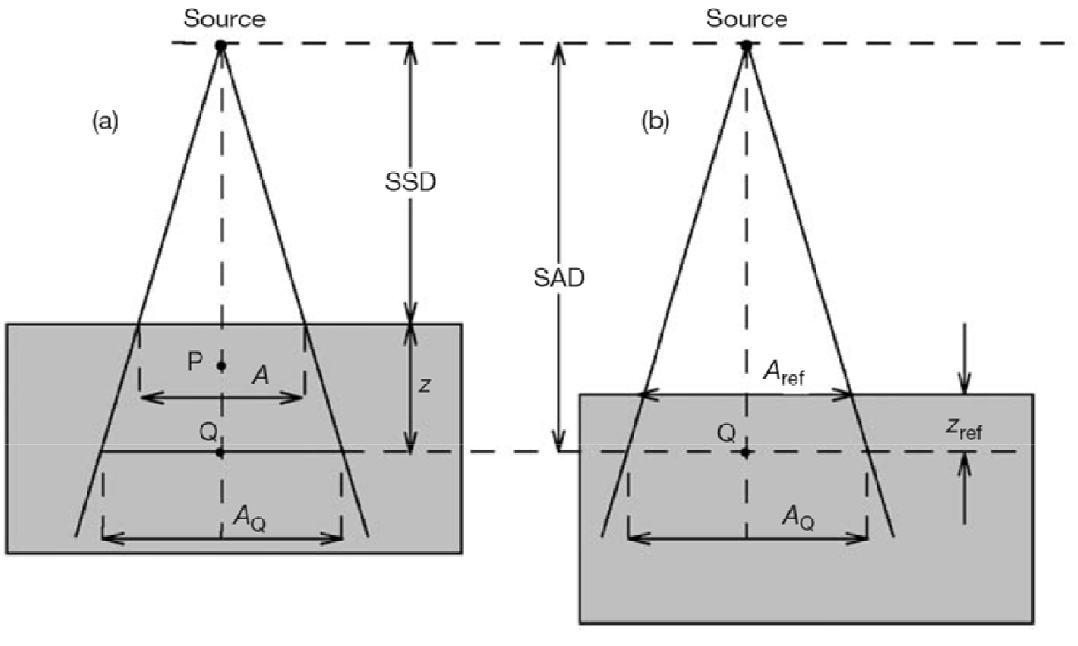
\includegraphics[scale=0.5]{figures/rtf.png}
  \caption{Conditions géométriques pour la mesure du l'indice de qualité}
  \label{fig_tpr}
\end{figure}

\subsection{Erreurs de positionnement}

Nous avons également réalisé des mesures pour mesurer l'impacte d'un mauvais positionnement de la chambre. Pour cela, nous avons appliqué un déplacement de 1 mm dans la direction latérale de part et d'autre du point de référence, puis 1 mm en profondeur au dessus et en dessous de ce même point. Dix mesures on été faites pour chaque énergie et chaque position pour ensuite calculer la charge moyenne. La dose est ensuite calculée selon le protocole TRS-398 de l'AIEA \cite{international2001iaea} puis un écart relatif est calculé entre la dose de référence et celle calculée avec le déplacement de 1 mm.

\subsection{Contrôle du débit de référence (TOP)}

Quotidiennement, un contôle qualité est réalisé sur les accélérateurs, communément appelé TOP. Ce contrôle permet de vérifier la dérive du débit dans le temps sur un faisceau fixe dans les conditions de référence (champ 10x10 cm$^2$, mesure faite à 10 cm de profondeur et DSD = 100 cm). La dose dans ces conditions est d'abord mesurée dans la cuve à eau, puis un facteur de passage entre l'eau et le bloc TOP est appliqué pour mesurer la dose dans le bloc lors des contrôles quotidiens. Ce facteur $f$ est défini comme suit :

\begin{equation}
  f = \dfrac{D_0}{M_0}
  \label{eq_facteur_top}
\end{equation}

Avec $D_0$ la dose mesurée dans les conditions de référence et $M_0$ la mesure dans la boîte à TOP.

\begin{figure}[h]
  \centering
  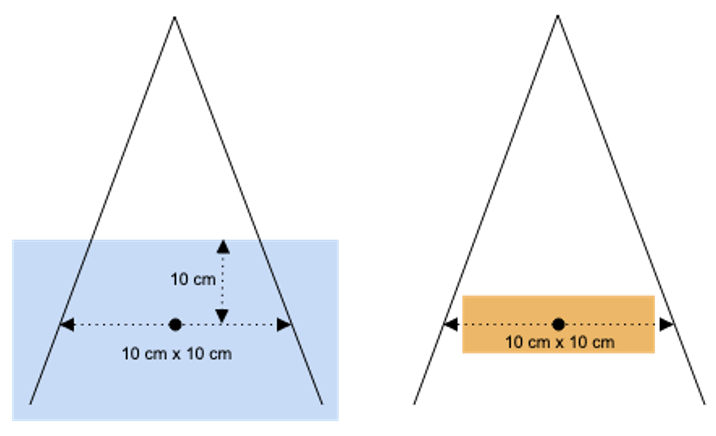
\includegraphics[scale=0.8]{figures/conditions_ref_top.png}
  \caption{Conditions de mesures de la dose absorbée dans la cuve à eau (à gauche) et dans le bloc TOP (à droite)}
  \label{fig_top}
\end{figure}

La dose du jour lors du contrôle qualité se calcule de la façon suivante :

\begin{equation}
  D_j = M_j \times \dfrac{D_0}{M_0} \times k_{TP} = M_j \times f \times k_{TP}
  \label{eq_top_jour}
\end{equation}

Avec $M_j$ la mesure du jour dans la boîte à TOP, $f = \frac{D_0}{M_0}$ le facteur de passage de la cuve à eau à la boîte à TOP et $k_{TP}$ le facteur de correction de la pression et de la température.

\newpage
\section{Résultats}
\subsection{Détermination des facteurs correctifs}

Le calcul des différents facteurs de correction de la mesure ont été calculés par les formules \ref*{eq_k_TP}, \ref*{eq_pol} et \ref*{eq_rec} (pour la pression et la température, la polarité et la recombinaison ionique) dont les résultats sont indiqués dans les tableaux \ref*{table_ktp} et \ref*{table_kpol}. Concernant la recombinaison ionique, les coefficients $a_0$, $a_1$ et $a_2$ sont indiqués dans le tableau \ref*{table_facteurs_krec}. Ces coefficients sont tirés du protocole TRP-398 de l'AIEA \cite{international2001iaea} représentés sur la figure \ref*{fig_krec}. L'ensemble des mesures de dose absolue ont été réalisées sur le Clinac 2.

\begin{table}[h]
  \centering
  \begin{tabular}{ccc}
    \toprule
    \textbf{Température (K)} & \textbf{Pression (hPa)} & $\mathbf{k_{TP}}$ \\
    \toprule
    21 & 1015 & 1,0017 \\
    \bottomrule
  \end{tabular}
  \caption{Calcul du $k_{TP}$}
  \label{table_ktp}
\end{table}


\begin{table}[h]
  \centering
  \begin{tabular}{c|cccc|cccc|}
  \cline{2-9}
                                                     & \multicolumn{4}{c|}{\textbf{X6}} & \multicolumn{4}{c|}{\textbf{X23}} \\ \hline
  \multicolumn{1}{|c|}{\textbf{Tension (V)}} & \textbf{400} & \textbf{100} & \textbf{-400} & \textbf{-100} & \textbf{400} & \textbf{100} & \textbf{-400} & \textbf{-100} \\ \hline
  \multicolumn{1}{|c|}{\textbf{Charge 1 (nC)}}       & 29,69  & 29,50  & 29,80  & 29,61 & 36,64  & 36,15  & 36,78  & 36,28  \\
  \multicolumn{1}{|c|}{\textbf{Charge 2 (nC)}}       & 29,70   & 29,52  & 29,82  & 29,59 & 36,62  & 36,10  & 36,75  & 36,25  \\
  \multicolumn{1}{|c|}{\textbf{Charge 3 (nC)}}       & 29,73  & 29,55  & 29,80  & 29,61 & 36,61  & 36,08  & 36,73  & 36,21  \\
  \multicolumn{1}{|c|}{\textbf{Charge moyenne (nC)}} & 29,71  & 29,52  & 29,81  & 29,60 & 36,62  & 36,11  & 36,75  & 36,25  \\ \hline
  \multicolumn{1}{|c|}{$\mathbf{k_{rec}}$}                & \multicolumn{4}{c|}{1,0020}      & \multicolumn{4}{c|}{1,0046}       \\
  \multicolumn{1}{|c|}{$\mathbf{k_{pol} \, 400 \, V}$}          & \multicolumn{4}{c|}{1,0019}      & \multicolumn{4}{c|}{1,0019}       \\
  \multicolumn{1}{|c|}{$\mathbf{k_{pol} \, 100 \, V}$}          & \multicolumn{4}{c|}{1,0014}      & \multicolumn{4}{c|}{1,0019}       \\ 
  \multicolumn{1}{|c|}{\textbf{Écart relatif} $\mathbf{k_{pol}}$ \textbf{\%}} & \multicolumn{4}{c|}{0,05} & \multicolumn{4}{c|}{0} \\
  \hline
  \end{tabular}
  \caption{Série de mesures avec la  pour le calcul du $k_{rec}$ et du $k_{pol}$ pour des faisceaux de photons de 6 MV et 23 MV (Clinac 2)}
  \label{table_kpol}
\end{table}



\begin{table}[h]
  \centering
  \begin{tabular}{cccc}
    \toprule
    $\mathbf{\frac{V_1}{V_2}}$ & $\mathbf{a_0}$ & $\mathbf{a_1}$ & $\mathbf{a_2}$\\
    \toprule
    4 & 1,022 & -0,363 & 0,341\\
    \bottomrule    
  \end{tabular}
  \caption{Facteurs tabulés correspondant au rapport $\frac{V_1}{V_2}$}
  \label{table_facteurs_krec}
\end{table}

\begin{figure}[h!]
  \centering
  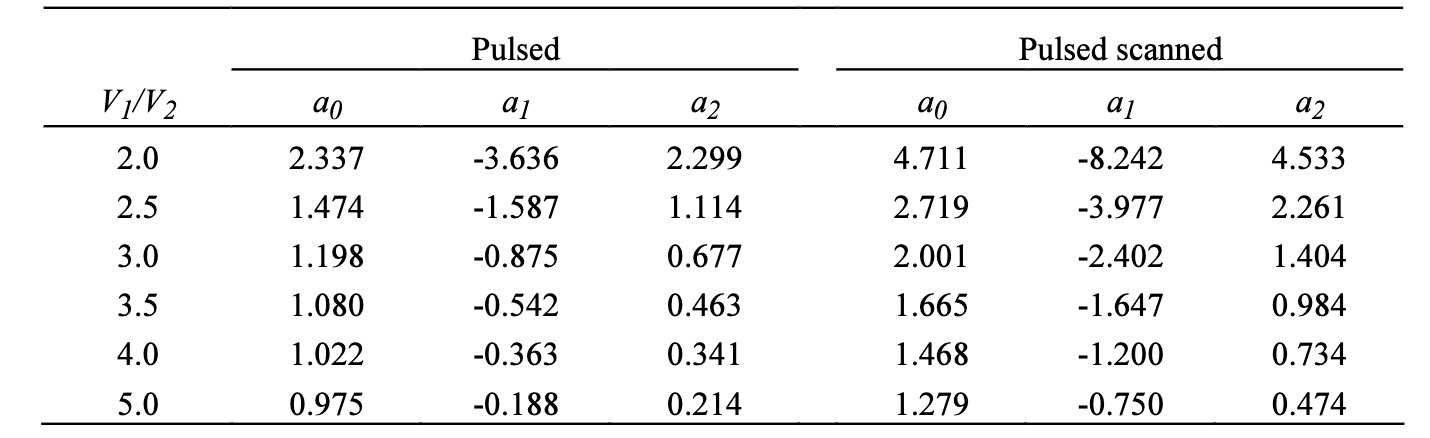
\includegraphics[scale=0.5]{figures/coeff_krec.png}
  \caption{Coefficients d'extrapolation pour le calcul du $k_{rec}$ par la technique des "deux tensions", en fonction du rapport $V_1/V_2$}
  \label{fig_krec}
\end{figure}

\newpage
\subsection{Mesure de l'indice de qualité}

L'indice de qualité est calculé pour les deux énergies disponibles sur le Clinac 2 (6 MV et 23 MV). Il a été calculé à l'aide de l'équation \ref*{eq_iq}. Nous avons réalisé 10 mesures de charge pour chaque énergie et chaque profondeur. Les valeurs moyennes ont été utilisées pour le calcul de l'indice de qualité, comme le montre le tableau \ref*{table_resultats_tpr}.

\begin{table}[h!]
  \centering
  \begin{tabular}{c|cc|cc|}
  \cline{2-5}
                                                                                     & \multicolumn{2}{c|}{\textbf{X6}} & \multicolumn{2}{c|}{\textbf{X23}} \\ \hline
  \multicolumn{1}{|c|}{\multirow{11}{*}{\textbf{Charge (nC)}}}                      & \textbf{10 cm}           & \textbf{20 cm}          & \textbf{10 cm}           & \textbf{20 cm}           \\ \cline{2-5} 
  \multicolumn{1}{|c|}{} & 29,70 & 19,70 & 36,58 & 28,60 \\
  \multicolumn{1}{|c|}{} & 29,66 & 19,67 & 36,57 & 28,54 \\
  \multicolumn{1}{|c|}{} & 29,66 & 19,66 & 36,58 & 28,51 \\
  \multicolumn{1}{|c|}{} & 29,69 & 19,70 & 36,57 & 28,52 \\
  \multicolumn{1}{|c|}{} & 29,66 & 19,66 & 36,58 & 28,52 \\
  \multicolumn{1}{|c|}{} & 29,63 & 19,65 & 36,62 & 28,53 \\
  \multicolumn{1}{|c|}{} & 29,63 & 19,66 & 36,58 & 28,53 \\
  \multicolumn{1}{|c|}{} & 29,63 & 19,68 & 36,60 & 28,53 \\
  \multicolumn{1}{|c|}{} & 29,64 & 19,65 & 36,58 & 28,54 \\
  \multicolumn{1}{|c|}{} & 29,69 & 19,66 & 36,59 & 28,53 \\
  \hline
  \multicolumn{1}{|c|}{\textbf{Charge moyenne   (nC)}}                               & 29,66           & 19,67          & 36,59           & 28,54           \\
  \hline
  \multicolumn{1}{|c|}{$\mathbf{TPR^{20}_{10}}$ \textbf{mesuré}}  & \multicolumn{2}{c|}{0,663}       & \multicolumn{2}{c|}{0,780}        \\
  \multicolumn{1}{|c|}{$\mathbf{TPR^{20}_{10}}$ \textbf{recette}} & \multicolumn{2}{c|}{0,664}       & \multicolumn{2}{c|}{0,781}        \\
  \multicolumn{1}{|c|}{\textbf{Écart relatif (\%)}}                                           & \multicolumn{2}{c|}{0,125}       & \multicolumn{2}{c|}{0,133}        \\ \hline
  \end{tabular}
  \caption{Résultats de la mesure du $TPR^{20}_{10}$ pour des faisceaux de photons de 6 MV et de 23 MV (Clinac 2)}
  \label{table_resultats_tpr}
\end{table}

\subsection{Mesure de la dose absolue de référence}

La mes sure de la dose absolue se base, dans nos manipulations, sur le protocole TRS-398 \cite{international2001iaea}. Les mesures de dose ont été réalisées sur les deux énergies 6 MV et 23 MV et pour deux chambres d'ionnisation étalonnées récemment : PTW  Farmer de 0,6 cm$^3$ et PTW Pinpoint de 0,03 cm$^3$ comme indiqué sans le tableau \ref*{table_dose_abs_resultats}.

\begin{table}[h!]
  \centering
  \begin{tabular}{c|cc|cc|}
  \cline{2-5}
                                             & \multicolumn{2}{c|}{\textbf{X6}}    & \multicolumn{2}{c|}{\textbf{X23}}   \\ \cline{2-5} 
                                             & \textbf{Farmer} & \textbf{Pinpoint} & \textbf{Farmer} & \textbf{Pinpoint} \\ \hline
  \multicolumn{1}{|c|}{\textbf{Charge moyenne (nC)}} & 29,66           & 0,675             & 36,59           & 0,8311            \\
  \multicolumn{1}{|c|}{\textbf{$\mathbf{N_{D_{eau},\, Q_0}}$ (Gy/nC)}} & 5,356$\times 10^{-2}$ & 2,344 & 5,356$\times 10^{-2}$ & 2,344                     \\
  \multicolumn{1}{|c|}{\textbf{$\mathbf{k_{Q,\, Q_0}}$}}       & \multicolumn{2}{c|}{0,9966}   & \multicolumn{2}{c|}{0,9767}                       \\
  \multicolumn{1}{|c|}{\textbf{Dose mesurée (Gy)}}   & 1,592           & 1,596             & 1,93            & 1,930             \\
  \multicolumn{1}{|c|}{\textbf{Dose recette (Gy)}}             & \multicolumn{2}{c|}{1,589}    & \multicolumn{2}{c|}{1,907}                        \\
  \multicolumn{1}{|c|}{\textbf{Écart relatif (\%)}}            & 0,18                  & 0,41  & 1,18                  & \multicolumn{1}{l|}{1,21} \\ \hline
  \end{tabular}
  \caption{Résultats de la dose absolue dans les conditions de référence avec les chambre Farmer et Pinpoint pour des faisceaux de 6 MV et 23 MV (Clinac 2)}
  \label{table_dose_abs_resultats}
\end{table}

\newpage
\subsection{Incertitudes}

Le tableau \ref*{table_incertitudes_abs} synthétise les incertitudes associées au calcul de la dose absolue dans les conditions de références.

\begin{table}[h]
  \centering
  \begin{tabular}{c|cc|cc|}
  \cline{2-5}
                                                           & \multicolumn{2}{c|}{\textbf{X6}} & \multicolumn{2}{c|}{\textbf{X23}} \\ \hline
  \multicolumn{1}{|c|}{\textbf{Type d'incertitude}}        & \textbf{A}      & \textbf{B}     & \textbf{A}      & \textbf{B}      \\ \hline
  \multicolumn{1}{|c|}{\textbf{Facteur d'étalonnage (\%)}} &                 & 0,55           &                 & 0,55            \\
  \multicolumn{1}{|c|}{$\mathbf{k_{Q,\,Q_0}}$ \textbf{(\%)}}                &                 & 1              &                 & 1               \\
  \multicolumn{1}{|c|}{$\mathbf{k_{TP}}$ \textbf{(\%)}}                  &                 & 0,28           &                 & 0,28            \\
  \multicolumn{1}{|c|}{$\mathbf{k_{pol}}$ \textbf{(\%)}}                 &                 & 0,08           &                 & 0,08            \\
  \multicolumn{1}{|c|}{$\mathbf{k_{rec}}$ \textbf{(\%)}}                 &                 & 0,11           &                 & 0,11            \\
  \multicolumn{1}{|c|}{\textbf{Charges collectées (\%)}}   & 0,09            &                & 0,04            &                 \\ \hline
  \multicolumn{1}{|c|}{\textbf{Total k=2 (\%)}}            & \multicolumn{2}{c|}{2,37}        & \multicolumn{2}{c|}{2,36}         \\ \hline
  \end{tabular}
  \caption{Incertitudes associées au calcul de la dose absolue pour des faisceaux de 6 MV et de 23 MV (Clinac 2)}
  \label{table_incertitudes_abs}
\end{table}

\subsection{Erreurs de positionnement}

\begin{table}[h]
  \centering
  \begin{tabular}{c|cc|cc|}
  \cline{2-5}
                                                           & \multicolumn{2}{c|}{\textbf{X6}} & \multicolumn{2}{c|}{\textbf{X23}} \\ \hline
  \multicolumn{1}{|c|}{\multirow{11}{*}{\textbf{Mesures brutes (nC)}}} & \textbf{1 mm} & \textbf{-1 mm} & \textbf{1 mm} & \textbf{-1 mm} \\ \cline{2-5} 
  \multicolumn{1}{|c|}{}                                   & 29,76           & 29,75          & 36,66           & 36,66           \\
  \multicolumn{1}{|c|}{}                                   & 29,76           & 29,79          & 36,66           & 36,66           \\
  \multicolumn{1}{|c|}{}                                   & 29,8            & 29,75          & 36,68           & 36,61           \\
  \multicolumn{1}{|c|}{}                                   & 29,78           & 29,8           & 36,69           & 36,63           \\
  \multicolumn{1}{|c|}{}                                   & 29,8            & 29,78          & 36,69           & 36,65           \\
  \multicolumn{1}{|c|}{}                                   & 29,79           & 29,8           & 36,7            & 36,65           \\
  \multicolumn{1}{|c|}{}                                   & 29,79           & 29,8           & 36,7            & 36,66           \\
  \multicolumn{1}{|c|}{}                                   & 29,78           & 29,79          & 36,71           & 36,66           \\
  \multicolumn{1}{|c|}{}                                   & 29,79           & 29,79          & 36,71           & 36,67           \\
  \multicolumn{1}{|c|}{}                                   & 29,8            & 29,78          & 36,7            & 36,67           \\ \hline
  \multicolumn{1}{|c|}{\textbf{Charge moyenne   (nC)}}     & 29,785          & 29,783         & 36,69           & 36,652          \\
  \multicolumn{1}{|c|}{\textbf{Écart-type (nC)}}           & 0,015           & 0,019          & 0,018           & 0,019           \\ \hline
  \multicolumn{1}{|c|}{\textbf{Dose (Gy)}}                 & 1,600           & 1,600          & 1,937           & 1,935           \\
  \multicolumn{1}{|c|}{\textbf{Incertitude absolue (Gy)}}  & 0,019           & 0,019          & 0,023           & 0,023           \\
  \multicolumn{1}{|c|}{\textbf{Incertitude relative (\%)}} & 1,182           & 1,182          & 1,178           & 1,182           \\
  \multicolumn{1}{|c|}{\textbf{Incertitude k=2 (\%)}}      & 2,364           & 2,365          & 2,356           & 2,363           \\
  \multicolumn{1}{|c|}{\textbf{Écart (mGy)}}               & 5,798           & 5,691          & 4,366           & 2,359           \\
  \multicolumn{1}{|c|}{\textbf{Écart relatif (\%)}}                   & 0,364           & 0,357          & 0,226           & 0,122           \\ \hline
  \end{tabular}
  \caption{Erreurs de positionnement engendré par un déplacement latéral de la chambre}
  \label{table_erreur_lat}
\end{table}

\begin{table}[h]
  \centering
  \begin{tabular}{c|cc|cc|}
  \cline{2-5}
                                                           & \multicolumn{2}{c|}{\textbf{X6}} & \multicolumn{2}{c|}{\textbf{X23}} \\ \hline
  \multicolumn{1}{|c|}{\multirow{11}{*}{\textbf{Mesures brutes (nC)}}} & \textbf{101 mm} & \textbf{109 mm} & \textbf{101 mm} & \textbf{109 mm} \\ \cline{2-5} 
  \multicolumn{1}{|c|}{}                                   & 29,53           & 29,88          & 36,46           & 36,76           \\
  \multicolumn{1}{|c|}{}                                   & 29,55           & 29,83          & 36,45           & 36,75           \\
  \multicolumn{1}{|c|}{}                                   & 29,56           & 29,88          & 36,46           & 36,76           \\
  \multicolumn{1}{|c|}{}                                   & 29,57           & 29,89          & 36,46           & 36,75           \\
  \multicolumn{1}{|c|}{}                                   & 29,54           & 29,87          & 36,47           & 36,75           \\
  \multicolumn{1}{|c|}{}                                   & 29,56           & 29,86          & 36,48           & 36,76           \\
  \multicolumn{1}{|c|}{}                                   & 29,56           & 29,88          & 36,47           & 36,76           \\
  \multicolumn{1}{|c|}{}                                   & 29,52           & 29,84          & 36,48           & 36,75           \\
  \multicolumn{1}{|c|}{}                                   & 29,57           & 29,87          & 36,48           & 36,76           \\
  \multicolumn{1}{|c|}{}                                   & 29,57           & 29,88          & 36,49           & 36,76           \\ \hline
  \multicolumn{1}{|c|}{\textbf{Charge moyenne   (nC)}}     & 29,553          & 29,868         & 36,470          & 36,756          \\
  \multicolumn{1}{|c|}{\textbf{Ecart-type (nC)}}           & 0,018           & 0,019          & 0,012           & 0,005           \\ \hline
  \multicolumn{1}{|c|}{\textbf{Dose (Gy)}}                 & 1,588           & 1,605          & 1,925           & 1,941           \\
  \multicolumn{1}{|c|}{\textbf{Incertitude absolue (Gy)}}  & 0,019           & 0,019          & 0,023           & 0,023           \\
  \multicolumn{1}{|c|}{\textbf{Incertitude relative (\%)}} & 1,182           & 1,182          & 1,179           & 1,181           \\
  \multicolumn{1}{|c|}{\textbf{Incertitude k=2 (\%)}}      & 2,364           & 2,365          & 2,357           & 2,361           \\
  \multicolumn{1}{|c|}{\textbf{Ecart (mGy)}}               & 6,667           & 10,258         & 7,249           & 7,850           \\
  \multicolumn{1}{|c|}{\textbf{ER (\%)}}                   & 0,418           & 0,643          & 0,375           & 0,406           \\ \hline
  \end{tabular}
  \caption{Erreurs de positionnement engendré par un déplacement en profondeur de la chambre}
  \label{table_erreur_profondeur}
\end{table}


\clearpage
\bibliography{biblio}
\addcontentsline{toc}{section}{Références}
\bibliographystyle{plain}
\nocite{*}

\end{document}